\documentclass[aspectratio=169,10pt,t,german,xcolor=table]{beamer}
\usepackage{../../common/beamer-cgs-lecture}

\title{Gem Illuminator}
\author{Pascal Lange, Sebastian Koall, Jennifer Stamm}
\institute{\translate{Hasso Plattner Institute}}
\date{WiSe~2014/2015}

\subtitle{Game Programming}
\titlegraphic{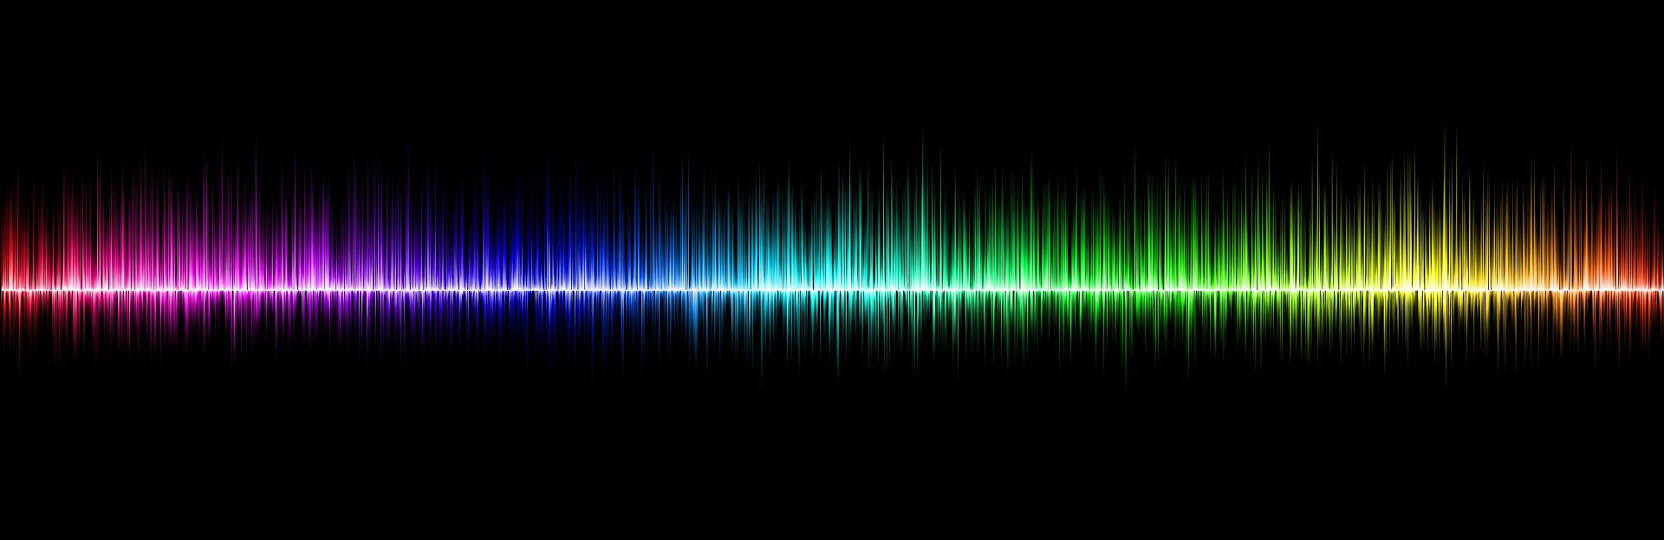
\includegraphics[width=\linewidth]{images/teaser}}

\begin{document}

% < 1m
\slidetitle
\section*{Abschlusspräsentation}

% 1m
\slideonetoonegraphics
{Motivation und Spielidee}
{images/start-situation}
{}
{images/lichteffekt-diffus-reflektion}
{}



% 3m
\begin{frame}{Demo}
	%TODO Aktueller Screenshot/Video
	\centering
	\includemedia[
	width=0.8\textwidth,height=0.8\textheight,
	activate=pageopen,
	flashvars={
		modestbranding=1 % no YT logo in control bar
		&autohide=1 % controlbar autohide
		&showinfo=0 % no title and other info before start
		&rel=0 % no related videos after end
		&vq=hd720
	},
	url % Flash loaded from URL
	]{}{http://www.youtube.com/v/krtvGjwKJaQ}
\end{frame}

% 1m
\begin{frame}{Entwicklungsumgebung}
\onetoone
{
	\begin{table}[h]
	\begin{tabular}{c|c|c|c}
		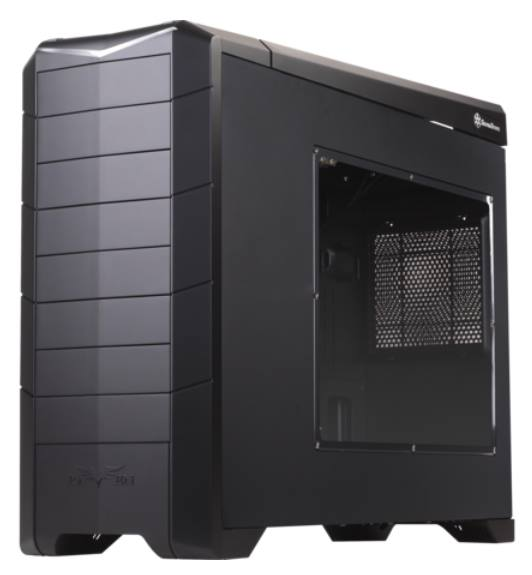
\includegraphics[width=\textwidth, height=0.1\textheight, keepaspectratio]{images/tower} &
		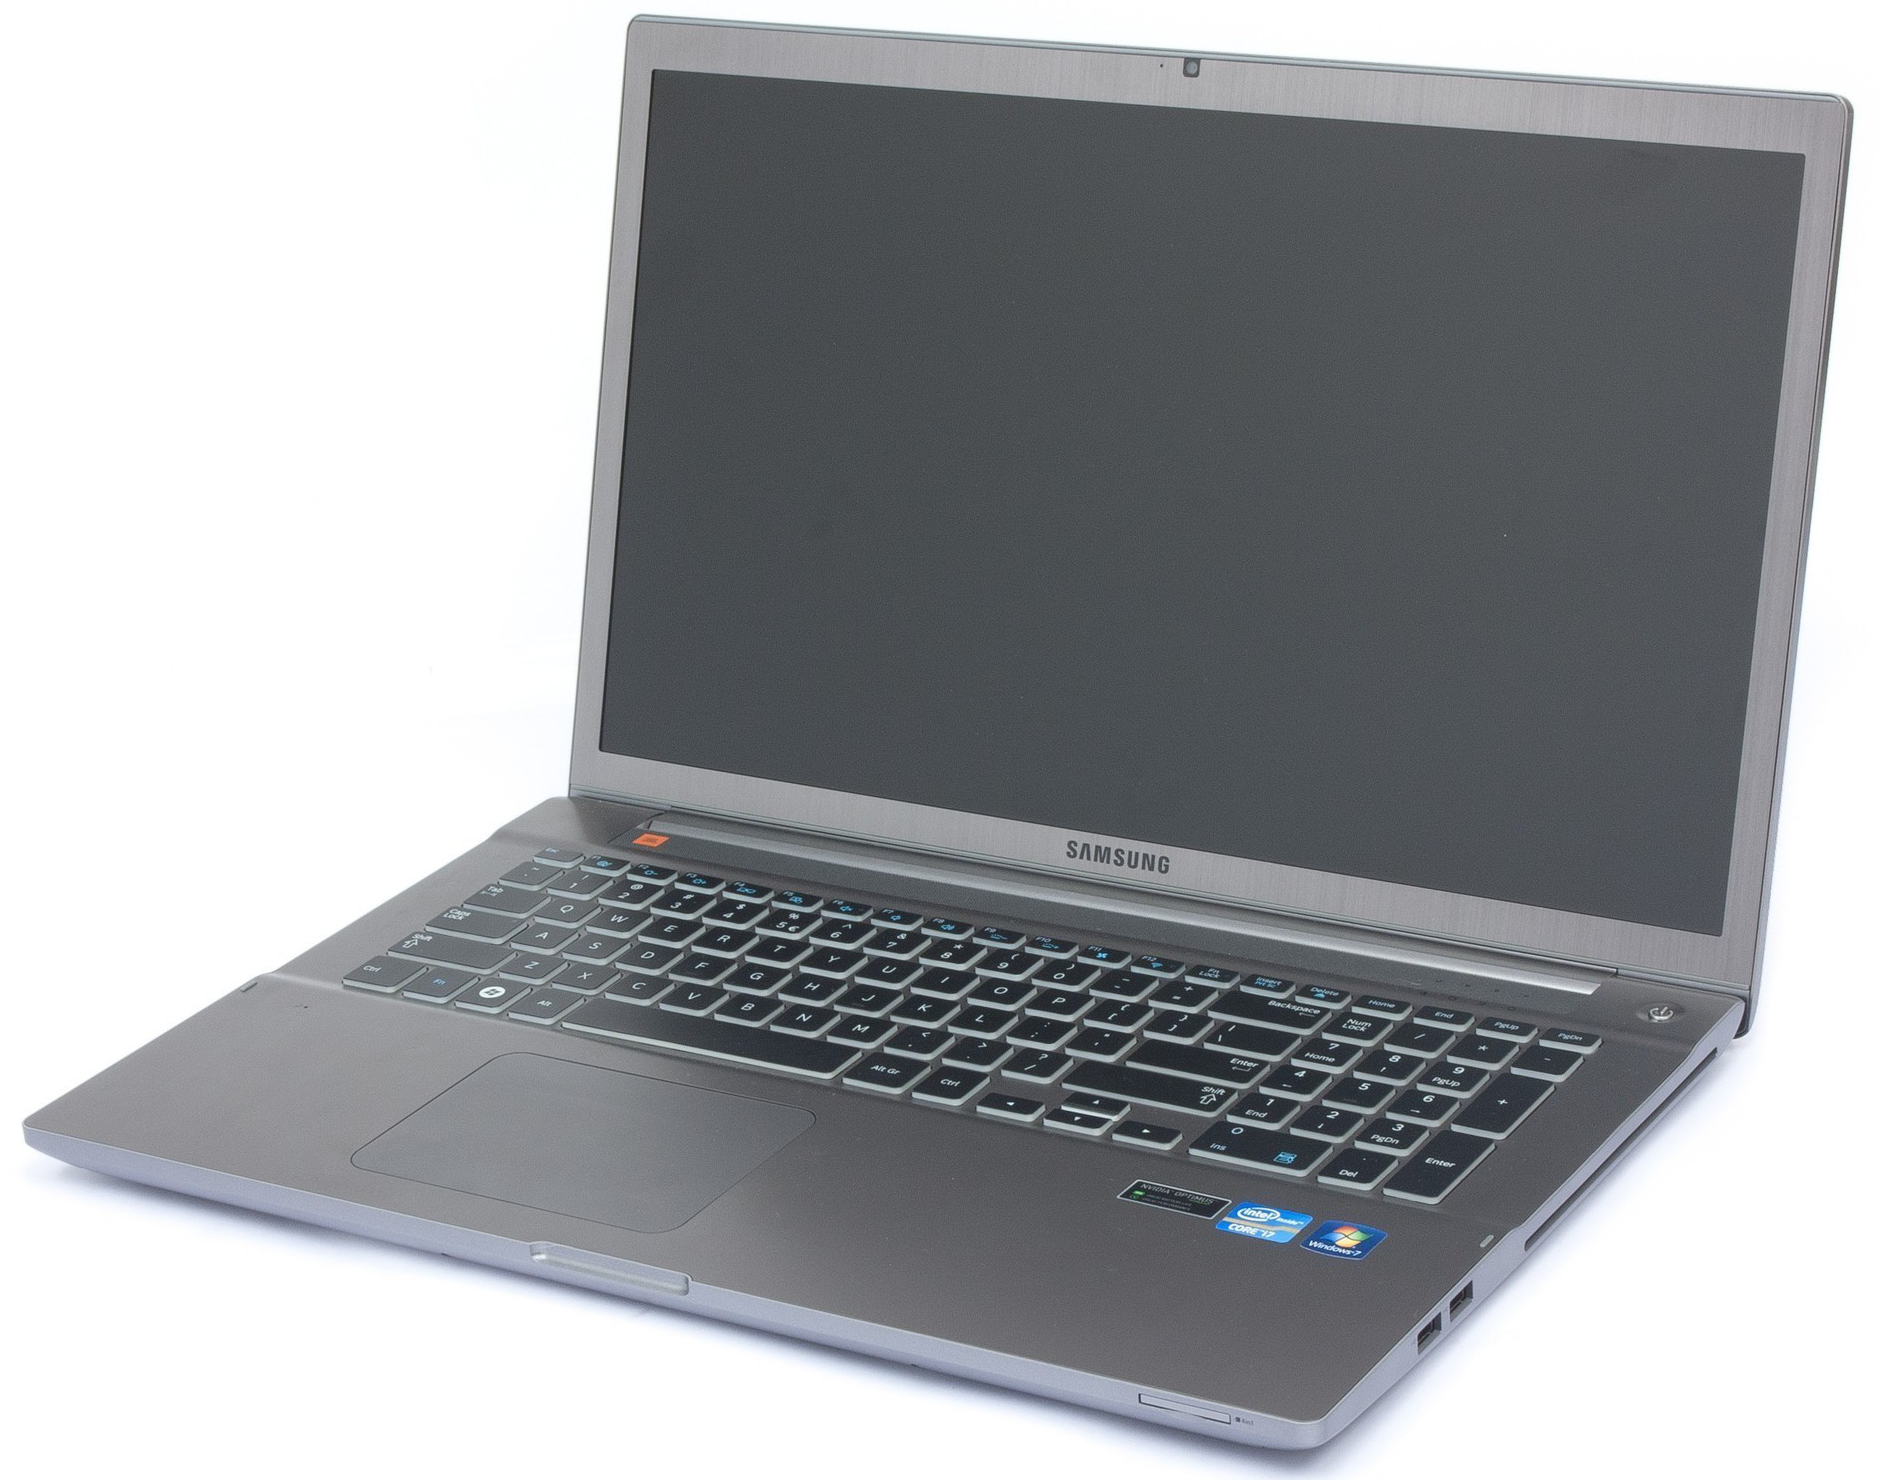
\includegraphics[width=\textwidth, height=0.1\textheight, keepaspectratio]{images/laptops} &
		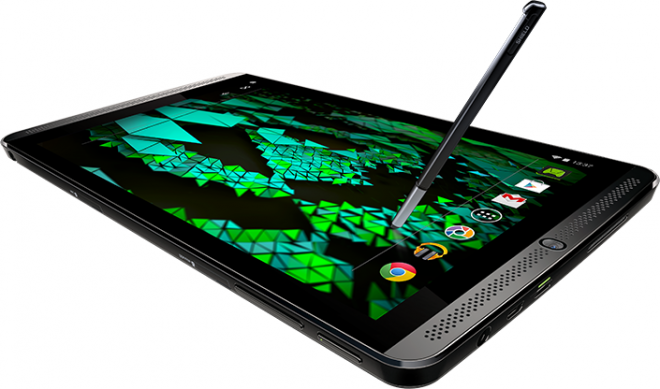
\includegraphics[width=\textwidth, height=0.1\textheight, keepaspectratio]{images/tablets} & 
		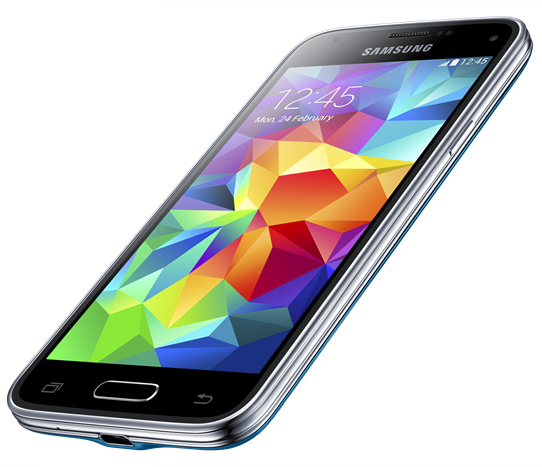
\includegraphics[width=\textwidth, height=0.1\textheight, keepaspectratio]{images/smartphones} \\ \hline
		3 & 3 & 2 & 2
	\end{tabular}
	\caption{Deployment auf 10 Geräten parallel}
	\end{table}
}
{
	\begin{figure}
		\centering
		
\includegraphics[width=\textwidth, height=0.18\textheight, keepaspectratio]{images/opengl_es_logo}
		\caption{Entwicklung mit OpenGL ES 2.0}
	\end{figure}
}
\begin{table}[h]
	\begin{tabular}{c|c|c|c|c}
		
\includegraphics[width=\textwidth, height=0.1\textheight, keepaspectratio]{images/AMD_Logo} &
		
\includegraphics[width=\textwidth, height=0.1\textheight, keepaspectratio]{images/nvidia-logo} &
		
\includegraphics[width=\textwidth, height=0.1\textheight, keepaspectratio]{images/Intel-logo}  &
		
\includegraphics[width=\textwidth, height=0.1\textheight, keepaspectratio]{images/powerVR-logo} &
		
\includegraphics[width=\textwidth, height=0.1\textheight, keepaspectratio]{images/qualcomm-logo} \\ \hline
		1 & 4 & 3 & 1 & 2
	\end{tabular}
	\caption{Verwendete Grafikkarten}
\end{table}
\end{frame}


% 2m
%\begin{frame}{Game Features}
	%Must-Haves, Should-Haves, Nice-To-Haves
	%\begin{itemize}
		%\item Start-Menü, Options-Menü mit Konfigurationsdatei, Ladebalken
		%\item Kristalllandschaftgenerierung mit Seeds
		%\item Verschiedene Kristalle
		%\item Wechselnde Lichtstrahlfarbe
		%\item Einfluss auf die Kristallfarbe
		%\item Reflektion bei Kollision
		%\item Pause-Button
		%\item Hintergrundmusik und Soundeffekte
		%\item Spielende und Highscore
	%\end{itemize}
%\end{frame}

\begin{frame}[c,plain]
	\begin{tikzpicture}[remember picture,overlay]
	\node[at=(current page.center)]
	{
		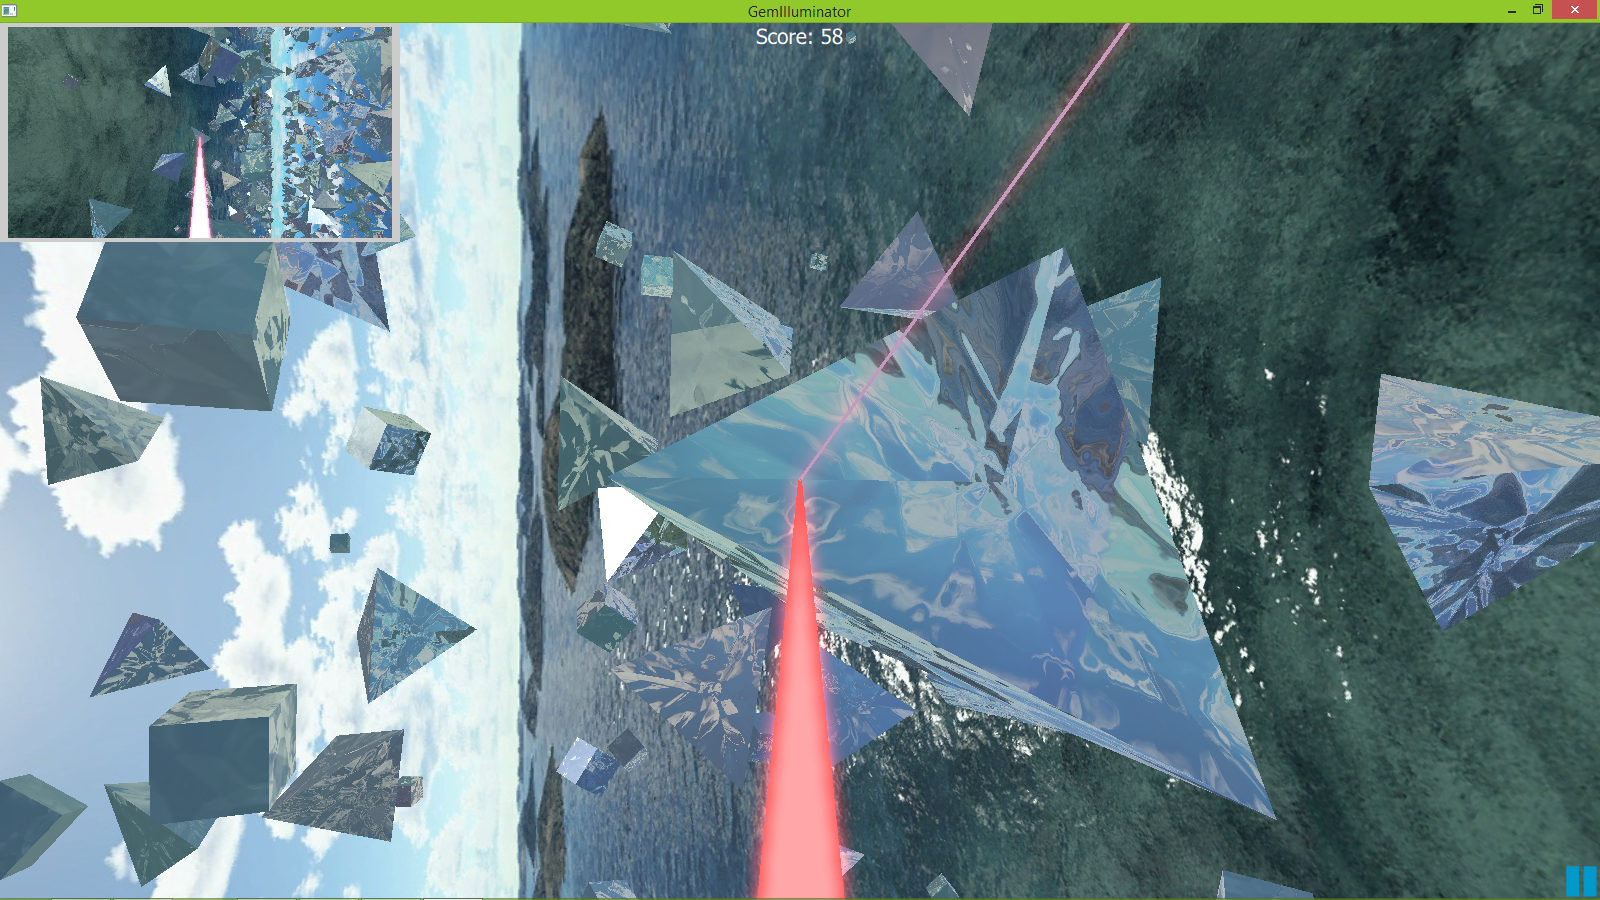
\includegraphics[width=\paperwidth, height=\paperheight]{images/screen}
	};
	\end{tikzpicture}	
	%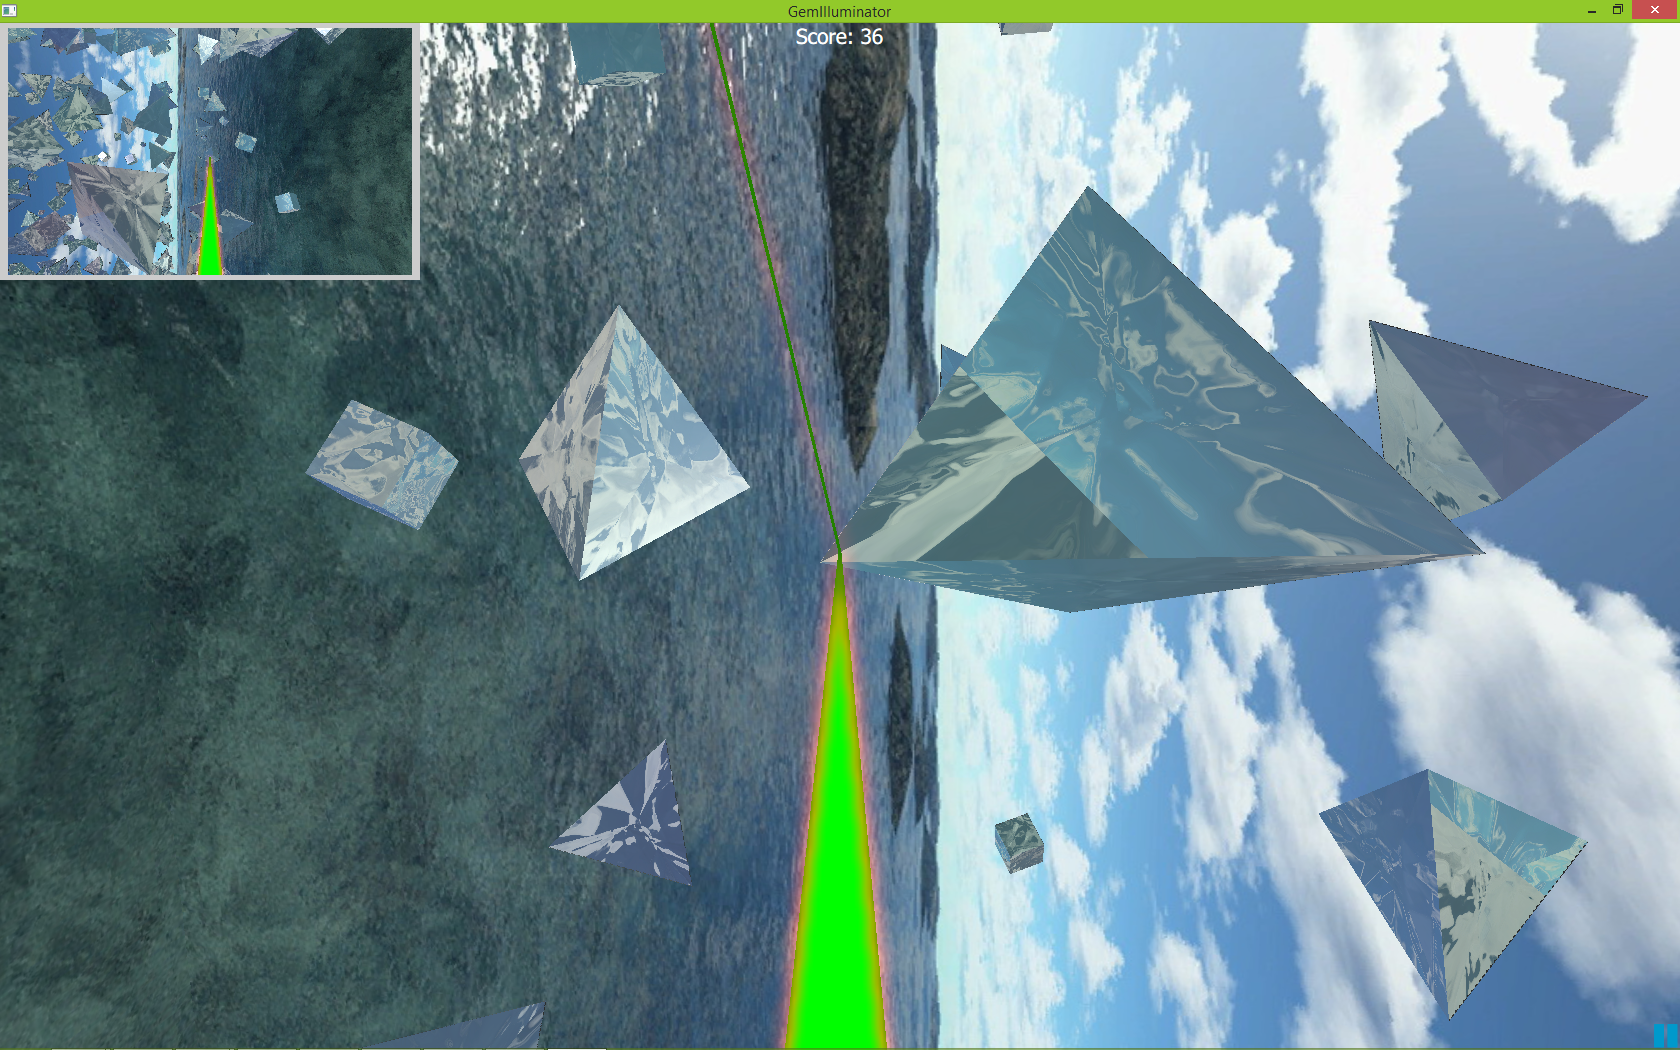
\includegraphics[width=\paperwidth]{images/screen-final}
\end{frame}

% 2m
\slideonetoone
{Computergraphic Features}
{
	\begin{figure}
		\centering
		\subcaptionbox{Environment Mapping}{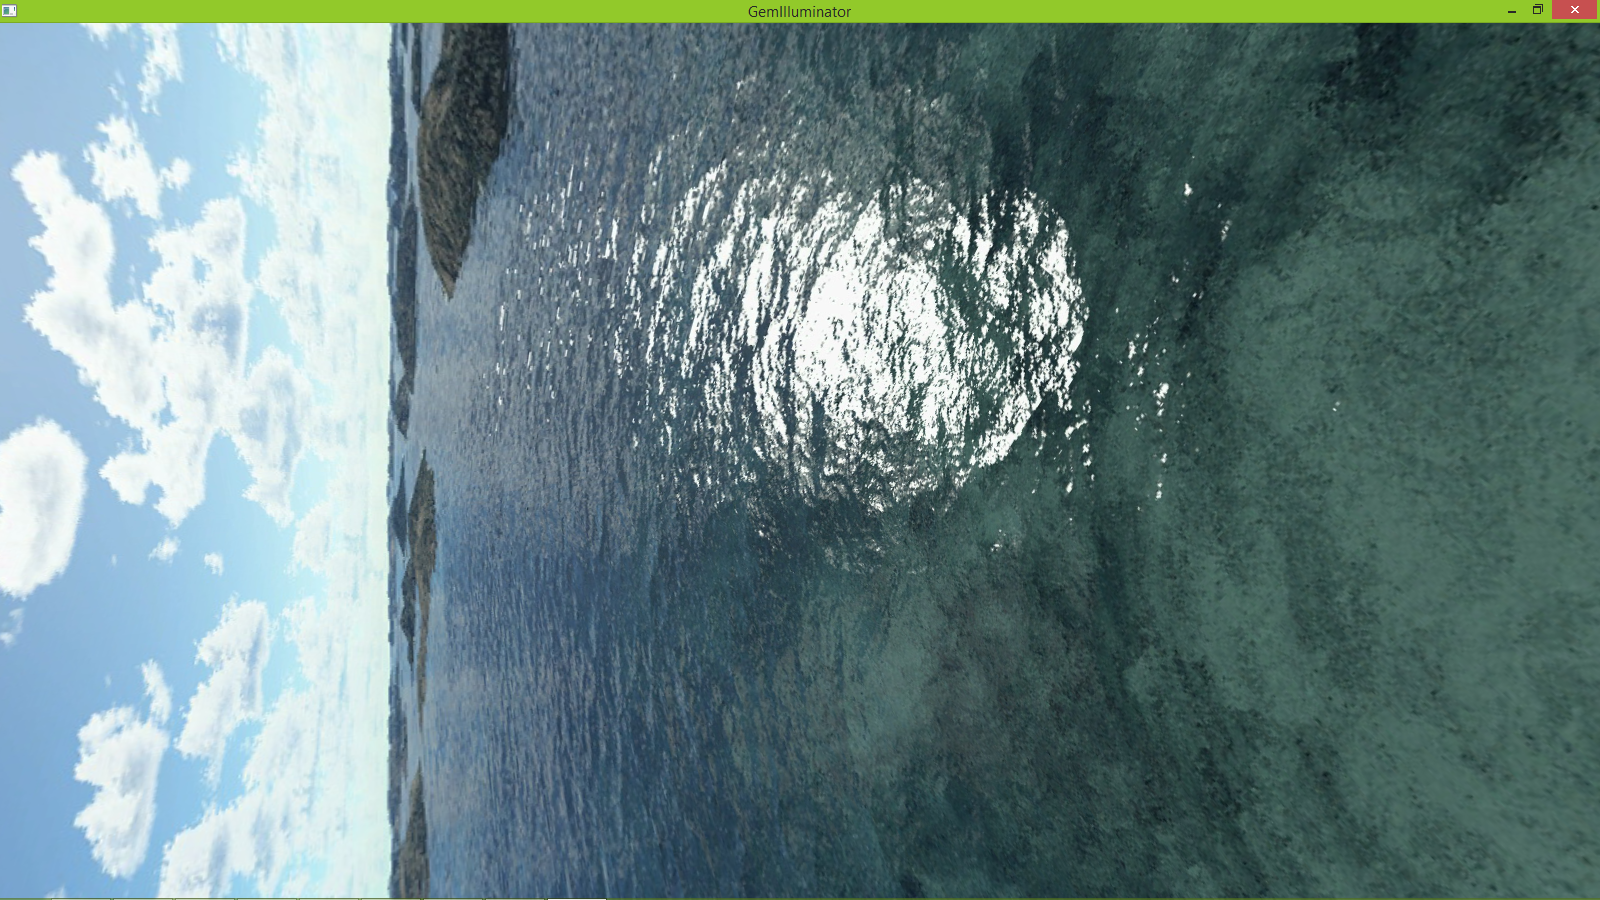
\includegraphics[width=\textwidth, height=0.3\textheight, keepaspectratio]{images/envmap}}
		\subcaptionbox{Preview-Window}{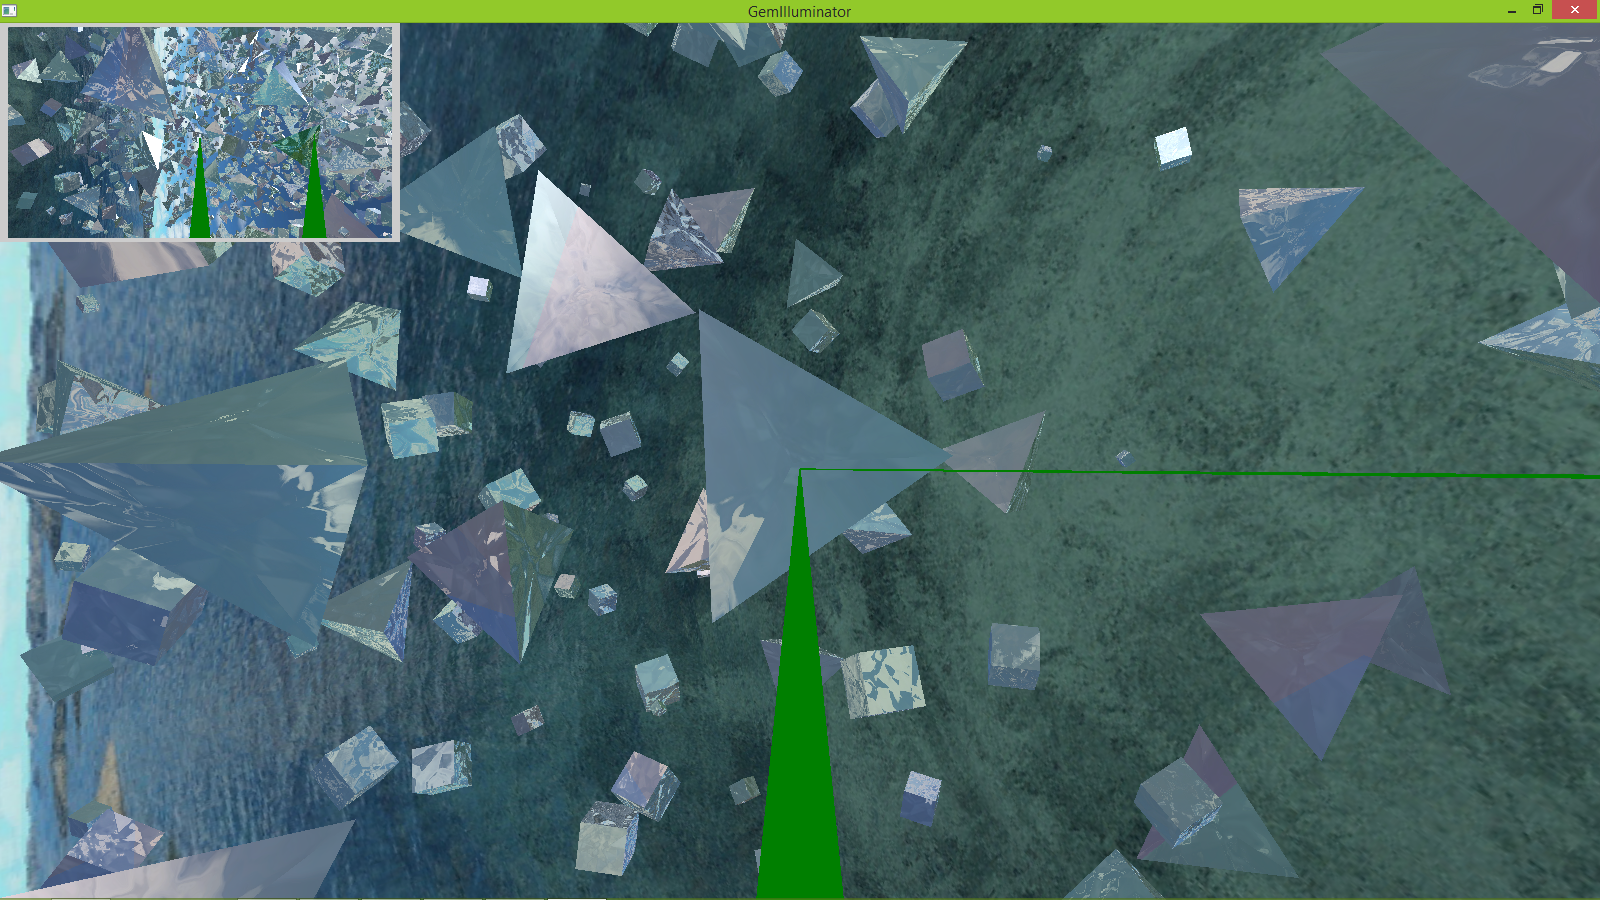
\includegraphics[width=\textwidth, height=0.3\textheight, keepaspectratio]{images/previewwindow}}
	\end{figure}
}
{
	\begin{figure}
		\centering
		\subcaptionbox{Licht- und Kristalleffekte}{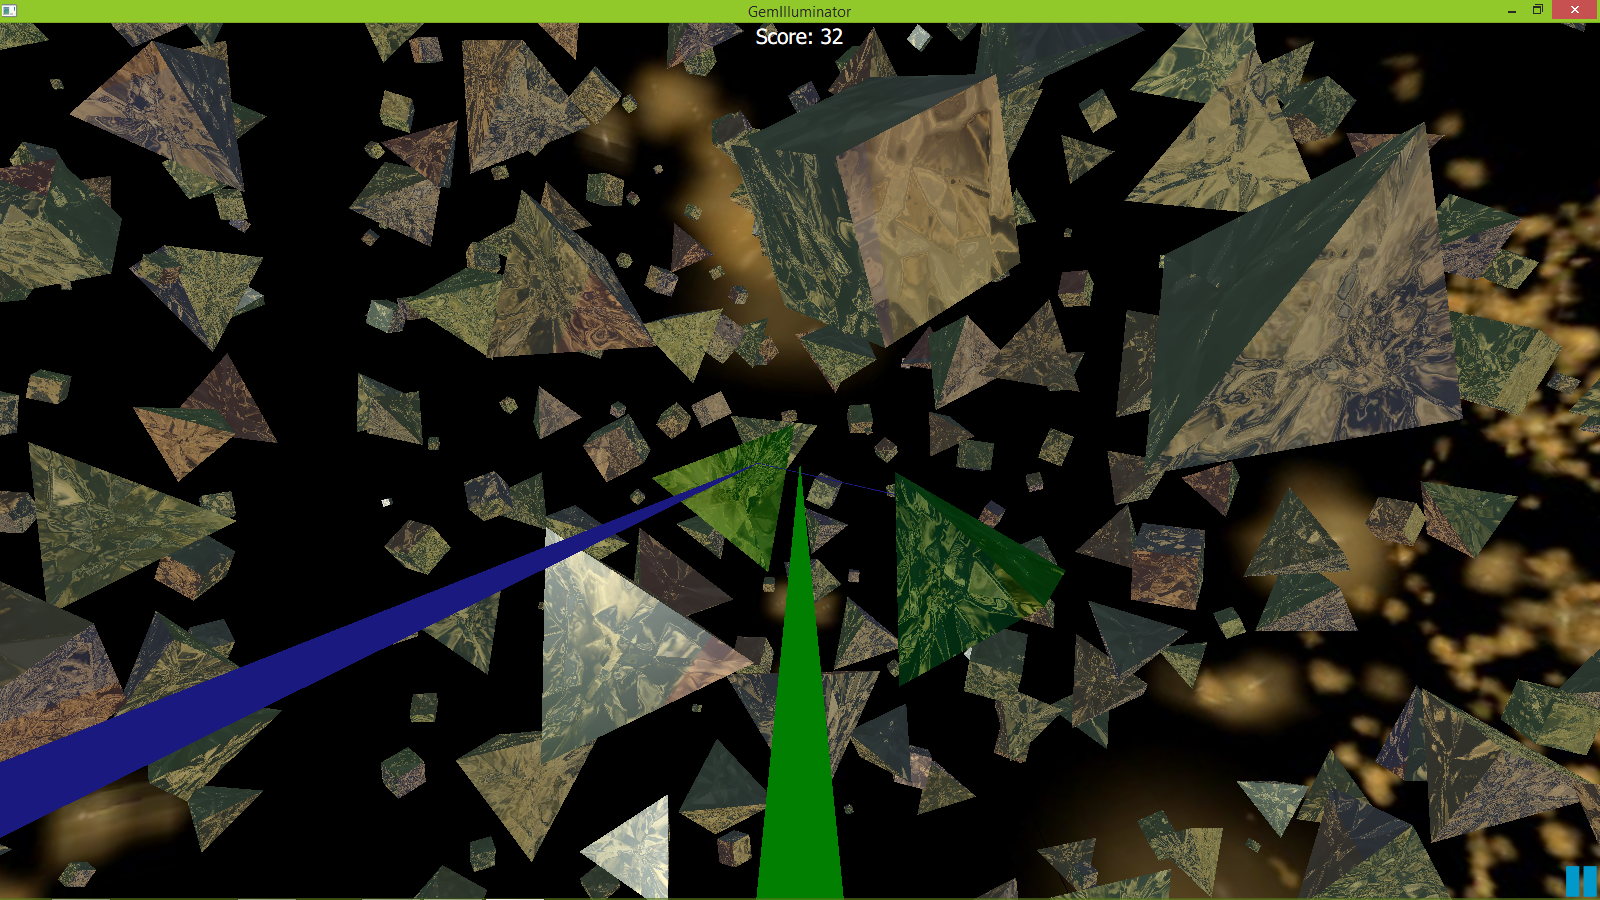
\includegraphics[width=\textwidth, height=0.3\textheight, keepaspectratio]{images/kristalleffekt}}
		\subcaptionbox{Glow-Effekt}{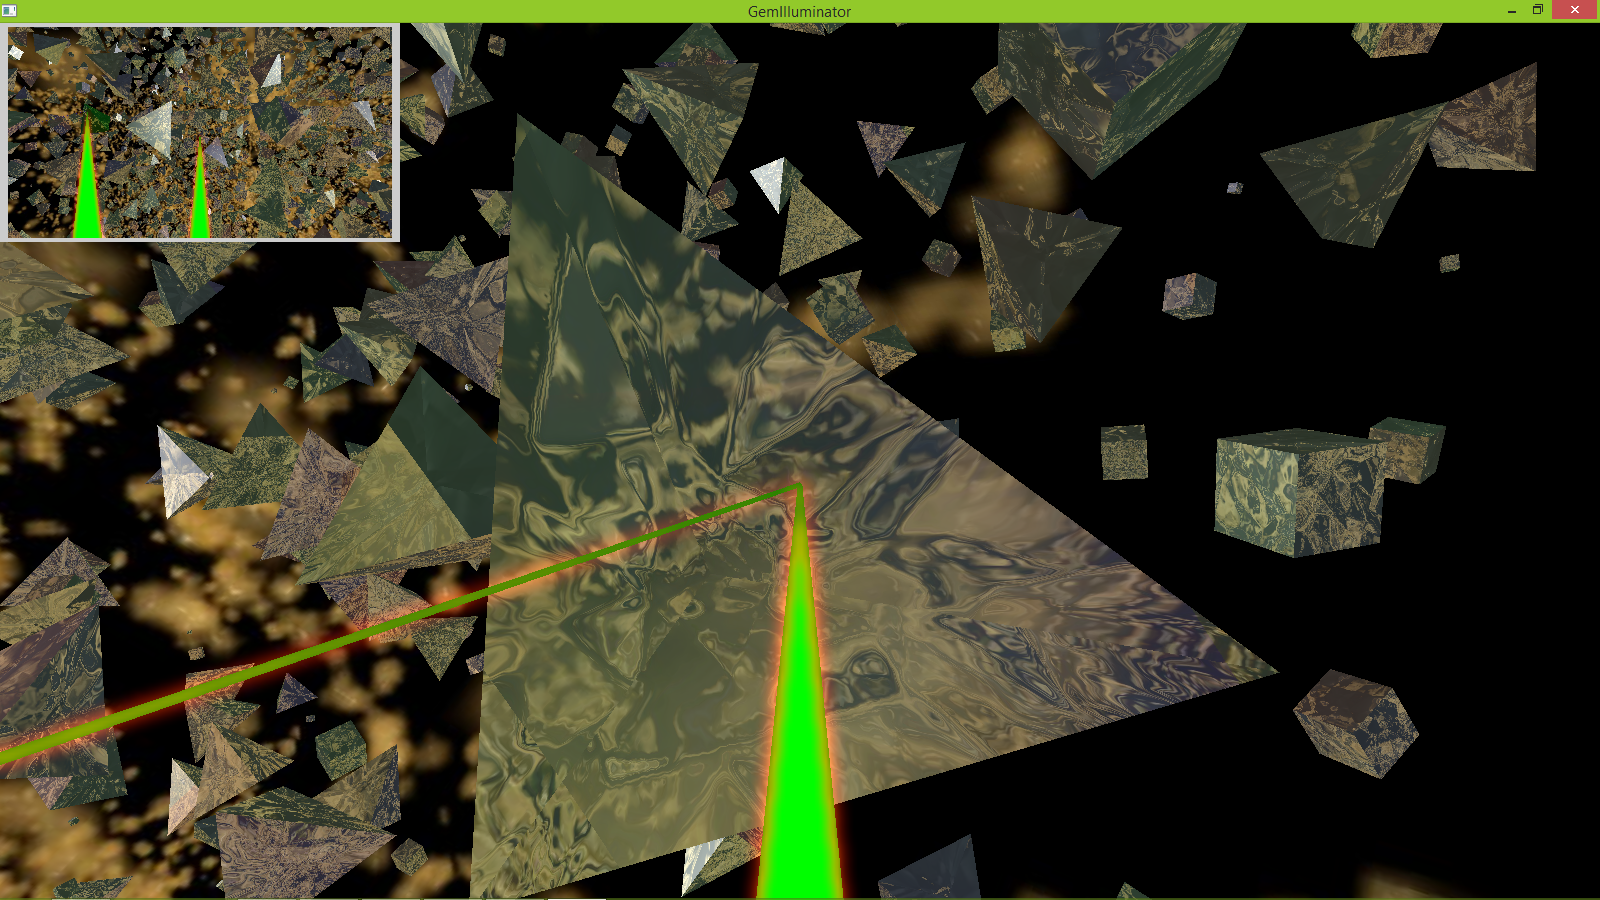
\includegraphics[width=\textwidth, height=0.3\textheight, keepaspectratio]{images/glow}}
	\end{figure}
}

% 2m
\slidegraphic
{Preview Window \& Glow}
{images/glowEffekt_gpuTextures_scaled}
{Glow-Effekt durch Blurring mit Gauss-Filter (Filterkerngröße $5\times 5$)}

% 1m
\begin{frame}{Architektur -- Zwischenstandspräsentation}
	\begin{figure}
		\centering
		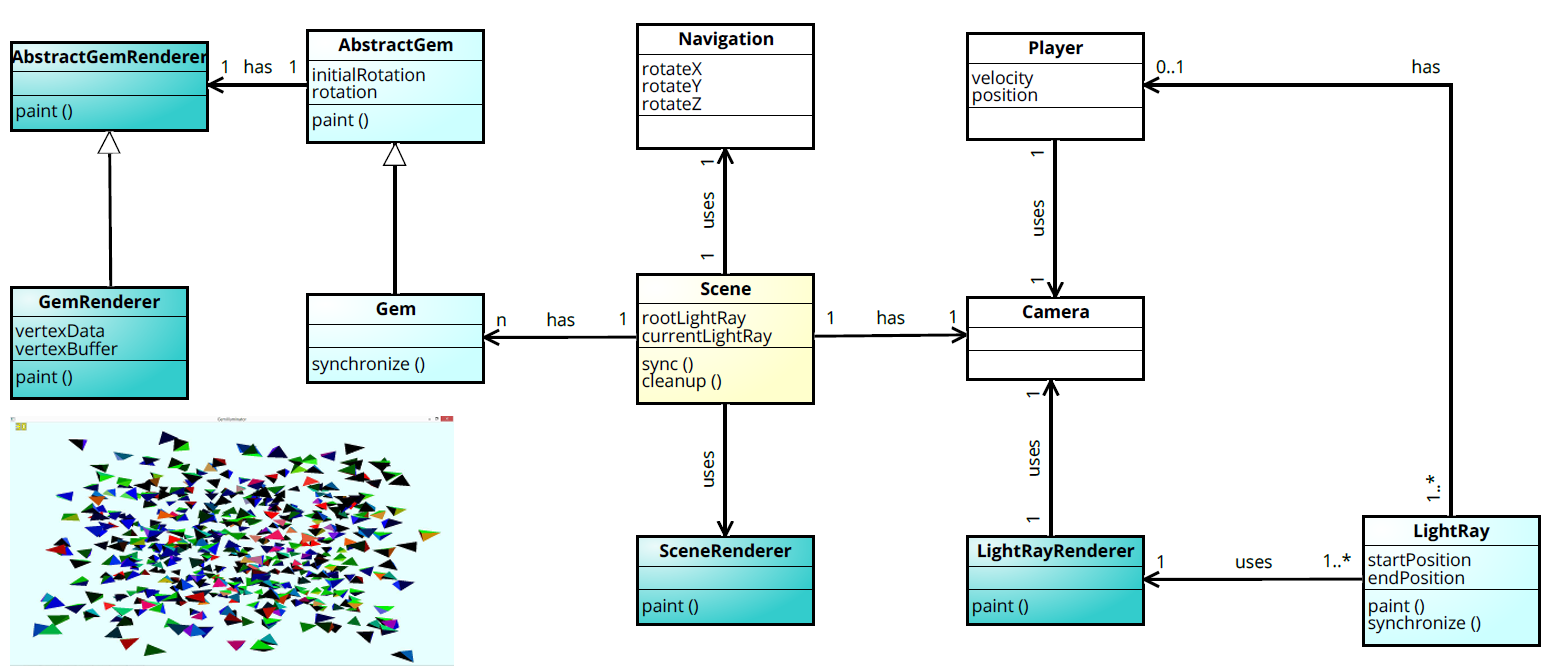
\includegraphics[width=\textwidth, height=0.8\textheight, keepaspectratio]{images/klassendiagramm}
	\end{figure}
\end{frame}

% 4m
\begin{frame}{Architektur -- Abschlusspräsentation}
	\begin{figure}
		\centering
		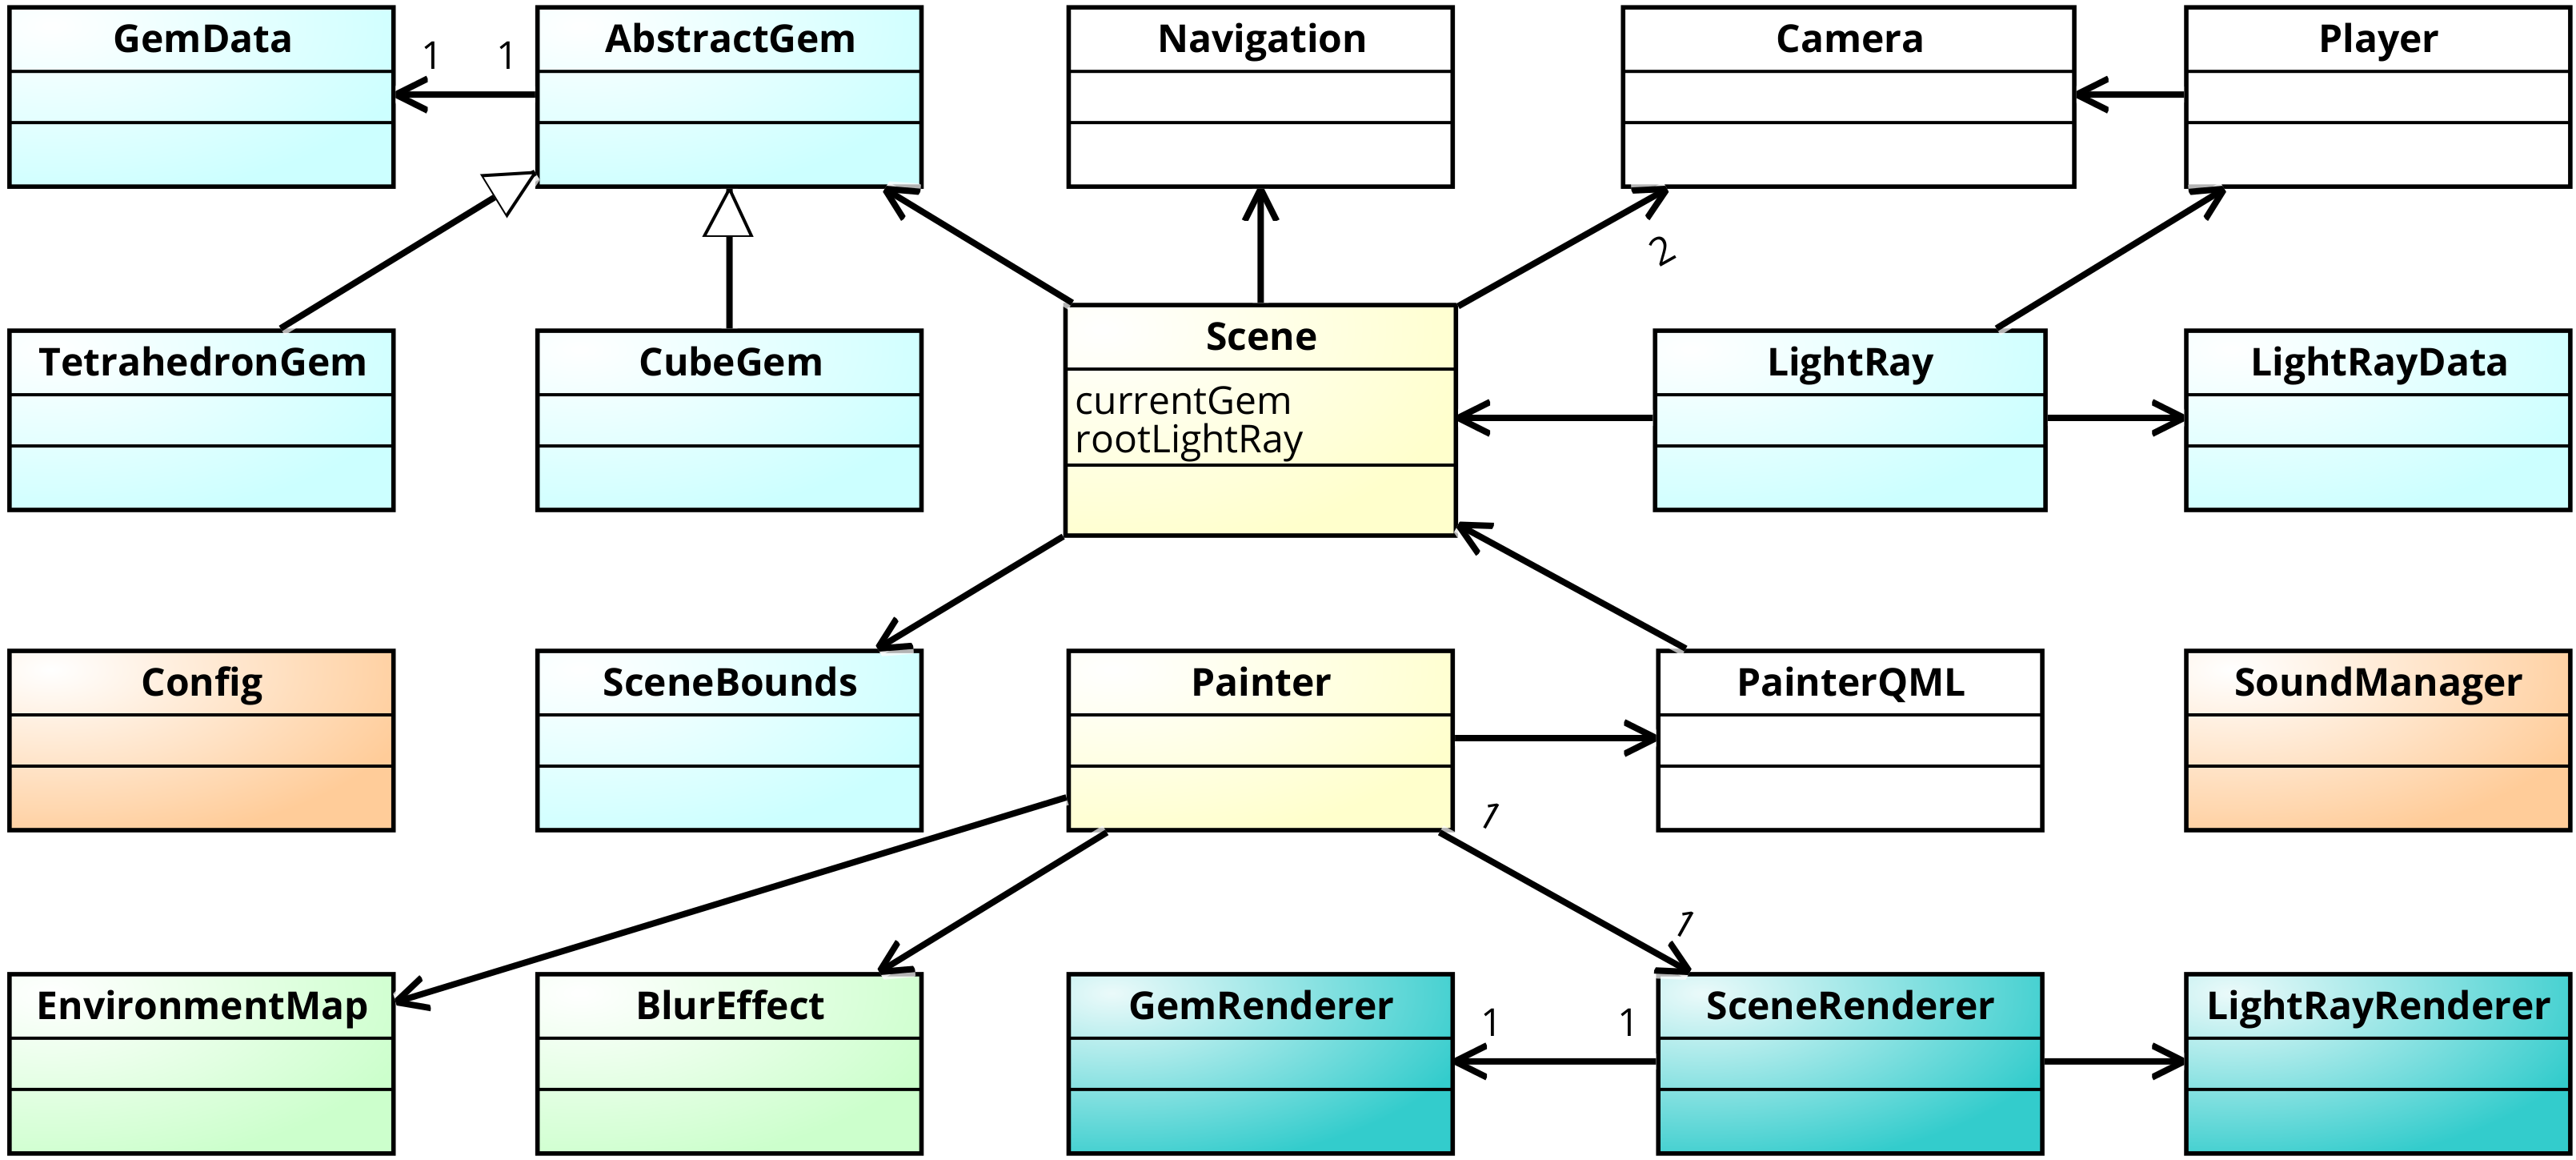
\includegraphics[width=\textwidth, height=0.8\textheight, keepaspectratio]{images/klassendiagramm-final}
	\end{figure}
\end{frame}

% 2m
\begin{frame}{Optimiertes Rendering}
	\begin{enumerate}
		\item Instance Drawing
		\vfill
		\item Attribut-Buffer + Textur + gl\_VertexID
		\vfill
		\item Attribut-Buffer + Textur + Index-Attribut
		\vfill
		\item Attribut-Buffer + Byte-Textur + Index-Attribut
		\vfill
		\item Attribut-Buffer + Byte-Textur/Float-Textur + Index-Attribut
	\end{enumerate}
\end{frame}

\slidegraphic
{Optimiertes Rendering}
{images/instancedDrawing}
{}

\begin{frame}{Fehler und Probleme}
	\centering
	\includemedia[
	width=0.8\textwidth,height=0.8\textheight,
	activate=pageopen,
	flashvars={
		modestbranding=1 % no YT logo in control bar
		&autohide=1 % controlbar autohide
		&showinfo=0 % no title and other info before start
		&rel=0 % no related videos after end
		&vq=hd720
	},
	url % Flash loaded from URL
	]{}{https://www.youtube.com/v/_bthr2lV3kw}
\end{frame}

% 1m
\begin{frame}{Fehler und Probleme}
	\begin{figure}
		\centering
		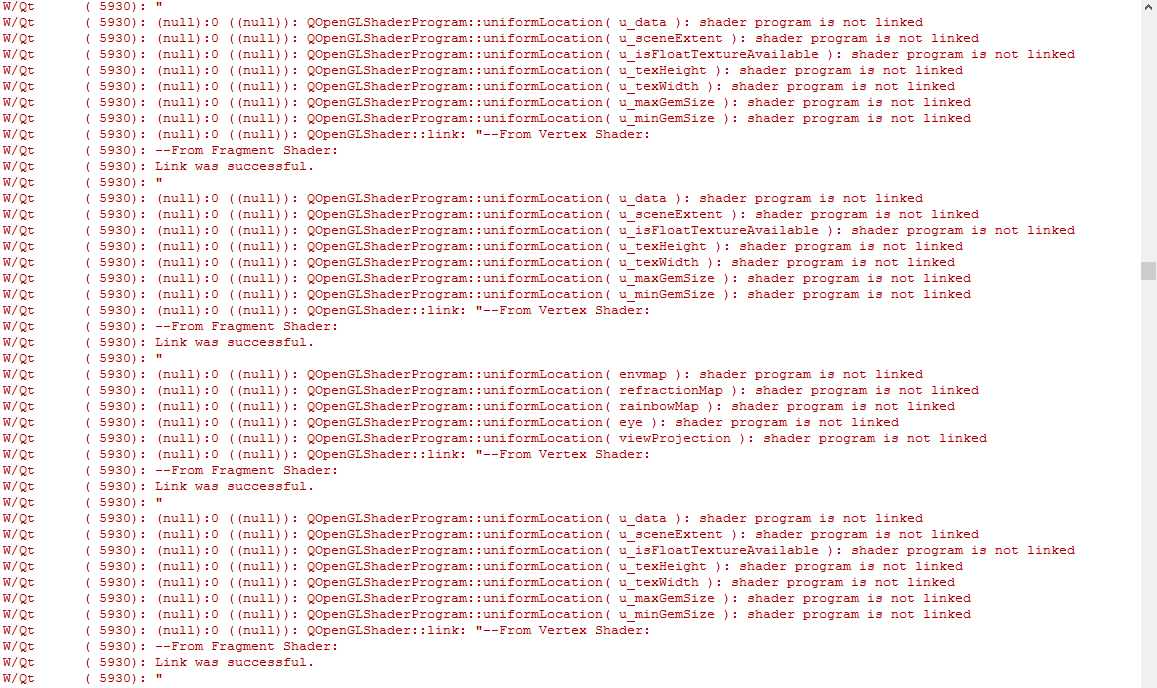
\includegraphics[width=\textwidth, height=0.2\textheight, keepaspectratio]{images/linkerrorsuccess}
		\caption{Vage Fehlermeldungen}
	\end{figure}
	\begin{figure}
		\centering
		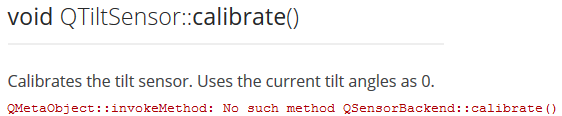
\includegraphics[width=\textwidth, height=0.17\textheight, keepaspectratio]{images/QMLCalibrate}
		 \caption{Inakkurate Dokumentation}
	\end{figure}
\end{frame}

% 1m
\begin{frame}{Lessons learned - Teamerfahrung}
	\onetoone
	{
	\begin{itemize}
		\item Abgleichen der Fähigkeiten, Erwartungen und Coding Styles
		\item Zufällig passendes Team
		\item Konstantes Arbeiten
	\end{itemize}
	}
	{
	\begin{itemize}
		\item Nachmittagstief
		\item Durchdachtes Spielkonzept vs. coole Spielidee
		\item Spaß
	\end{itemize}
	}
	\begin{figure}
		\centering
		\subcaptionbox{Zwischenstand}{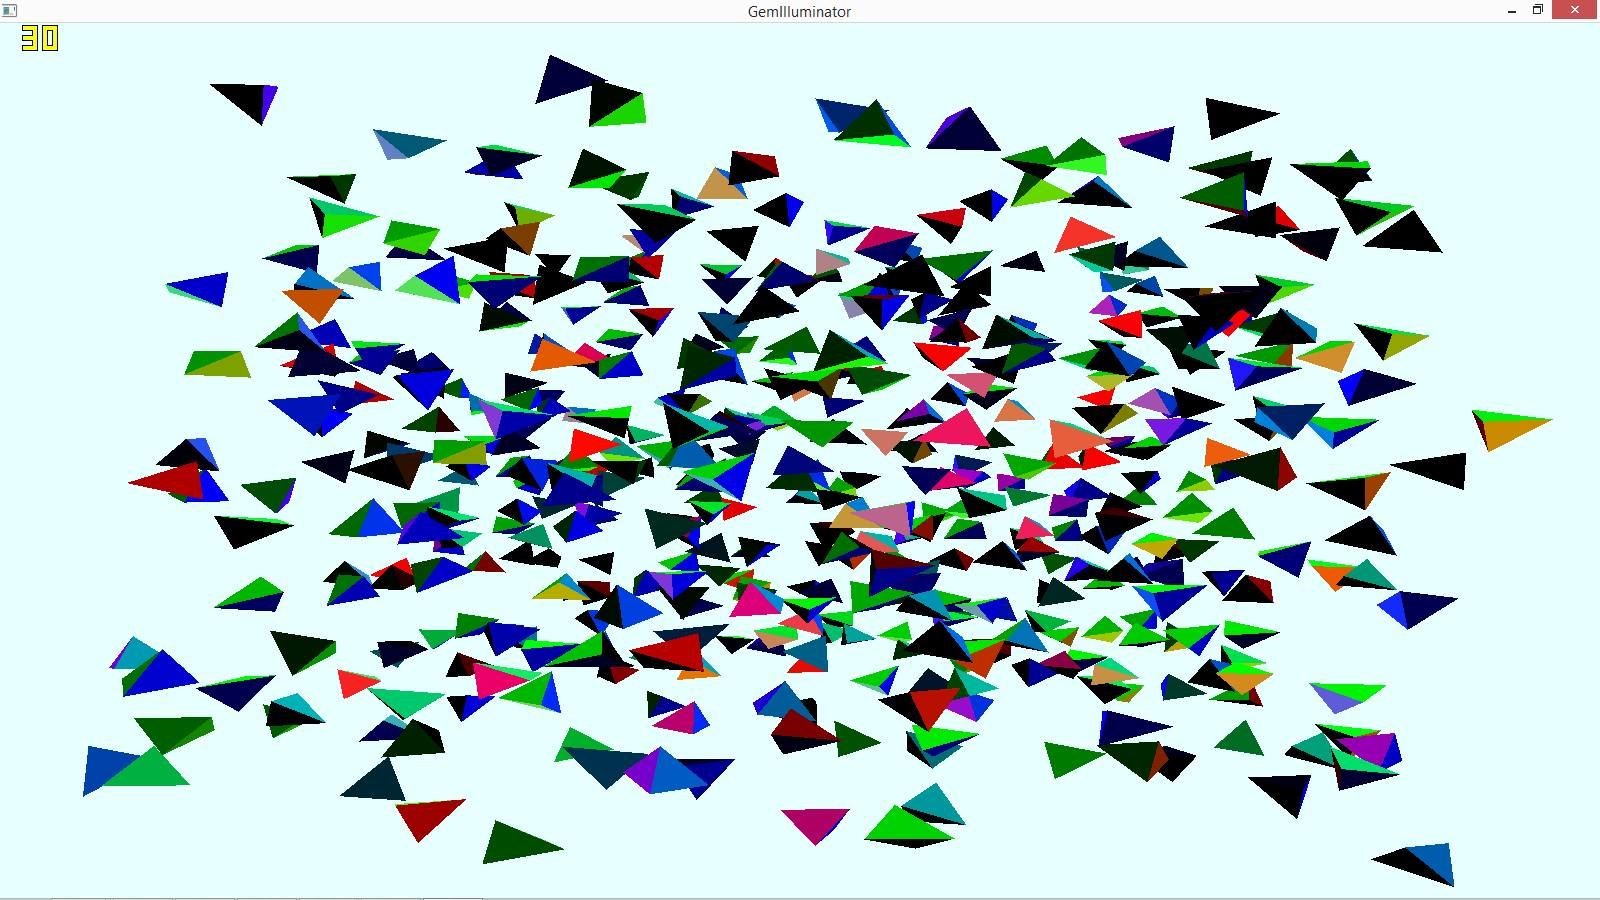
\includegraphics[width=\textwidth, height=0.45\textheight, keepaspectratio]{images/500_gems_intel}}
		\subcaptionbox{Finaler Stand}{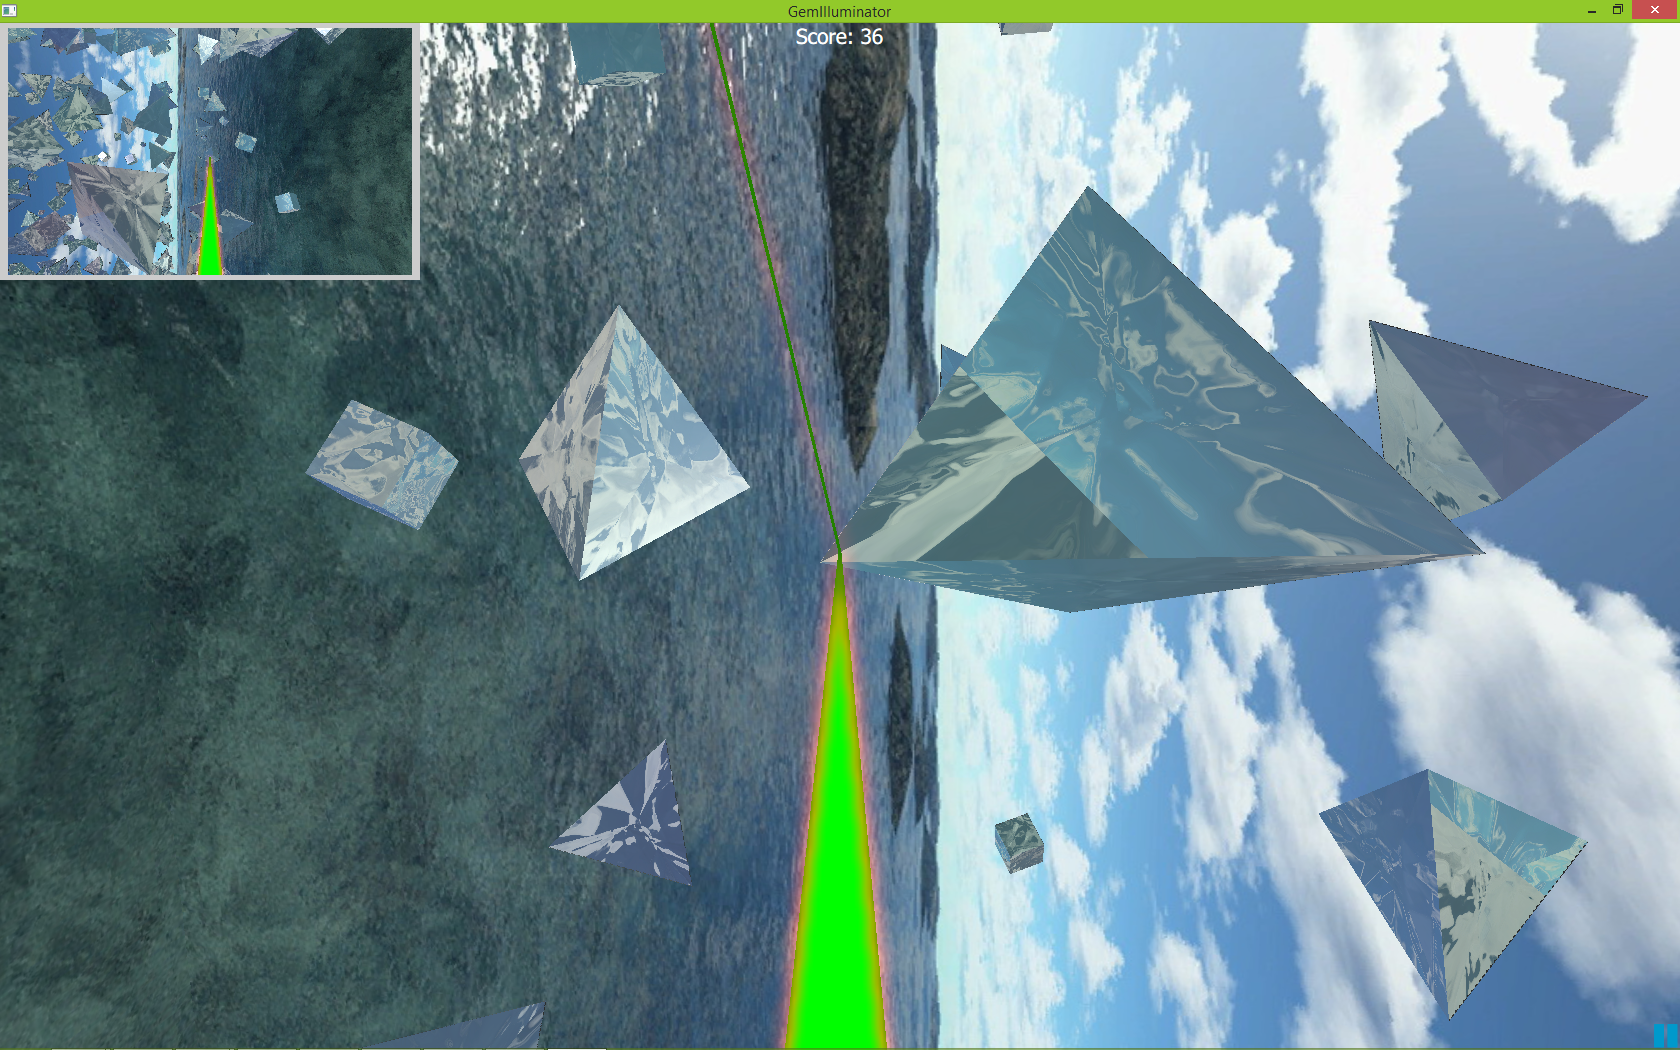
\includegraphics[width=\textwidth, height=0.45\textheight, keepaspectratio]{images/screen-final}}
	\end{figure}
\end{frame}

% 1m
\slidegraphic
{Lessons learned - OpenGL ES 2.0 und QML}
{images/time-graph}
{Es ist nicht unmöglich, aber es dauert.}

\nocite{*}
\begin{frame}[allowframebreaks]{Bibliographie}
  \bibliographystyle{apalike}
  \bibliography{../../references}
  \vfill
\end{frame}

\end{document}
